\subsection{Monitoraggio e Intervento}
L'utilizzo della suite \textbf{SciML.ai} e' stato fatto per l'integrazione
di un modello di Machine Learning in un sistema di monitoraggio e possibilmente di 
intervento. 

\subsubsection{Predizione}
Applicare un algoritmo di ML per predire l'andamento di un sistema non lineare dinamico 
senza avere una grande base di dati puo' risultare problematico e i risultati possono risultare 
poco affidabili. Lo sviluppo di tecniche che congiungono la modellazione puramente matematica
alla flessibilita' delle reti neurali ha permesso di sviluppare approcci \emph{data-driven domain-specific} 
\cite{rackauckas2020universal} \cite{Kim_2021} \cite{dandekar2022bayesian}
che permettono di ottenere risultati affidabili pur avendo una base di dati scarsa. 

\subsubsection*{UDE e Neural Network}
L'approccio iniziale al problema e' stato quello di definire una rete neurale con cui andare
ad effettuare le predizioni che serviranno per determinare l'andamento delle curve e i possibili
interventi.

\begin{minipage}{\linewidth}
	\centering
	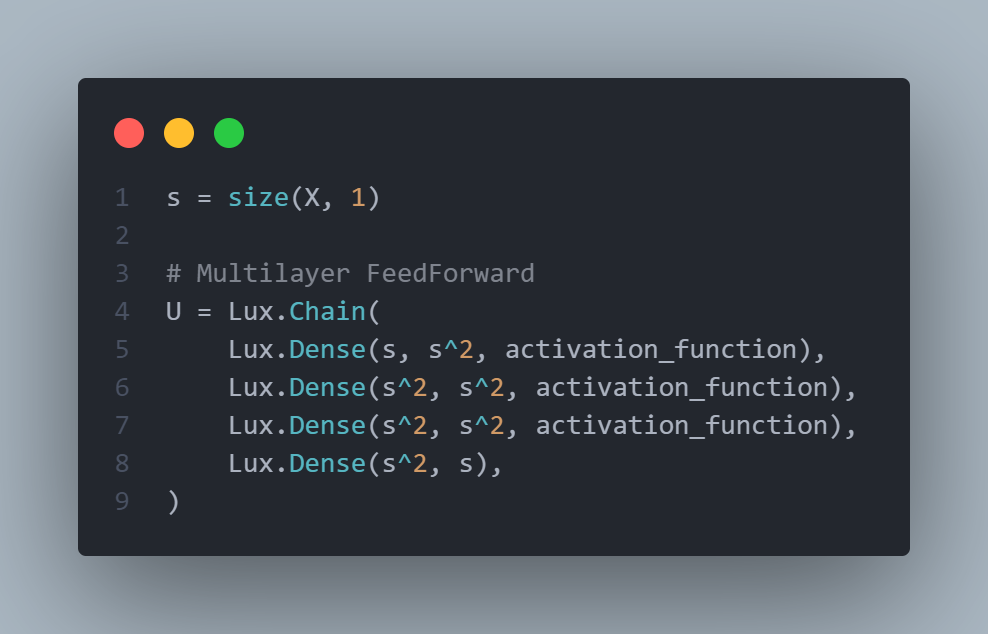
\includegraphics[width=\textwidth]{img/lux_nn.png}
	\captionof{figure}{Definizione della rete neurale utilizzando la libreria Lux.jl \cite{pal2023lux}}
	\label{fig:lux_nn}
\end{minipage}

L'idea principale alla base dell'approccio delle \textbf{Neural ODE} e' quello di accorpare
due approcci per ottenere il meglio da entrambi. Partendo ad analizzare la definizione della 
rete neurale, si puo' osservare come sia del tipo \emph{FeedForward}. L'approccio utilizzato per 
definire quanti \emph{hidden nodes} dovessero essere presenti all'interno di ogni \emph{layer} 
della rete e' basato sul numero di equazioni che si vogliono ricavare. Questo numero viene ricavato 
dai dati in input, che sono nella forma \textbf{DataFrame} e che vengono successivamete convertiti 
in una forma di tipo \textbf{Array}. Le righe che compongono la matrice \textbf{X} sono le mie equazioni
incognite.

Per cui si ottiene che il numero di nodi in input e output sara' esattamente il numero 
di equazioni incognite, mentre il numero di hidden nodes sara' pari al quadrato di quest'ultimo.
La scelta di questo valore ricade principalmente sul fatto che si sta analizzando un sistema SEIRD, 
quindi a 5 stati (equazioni). Avere 25 hidden nodes per ogni hidden layer mi e' sembrata una scelta 
ragionevole. Cosi' come avere un numero di hidden layer decisamente ristretto. 

L'idea alla base e' quella comunque di avere un modello molto snello, sia in memoria che in 
tempo di computazione, che permetta di arrivare ad avere risultati affidabili con un numero 
contenuto di iterazioni, senza richiede al contempo un elevato quantitativo di memoria.

\begin{minipage}{\linewidth}
	\centering
	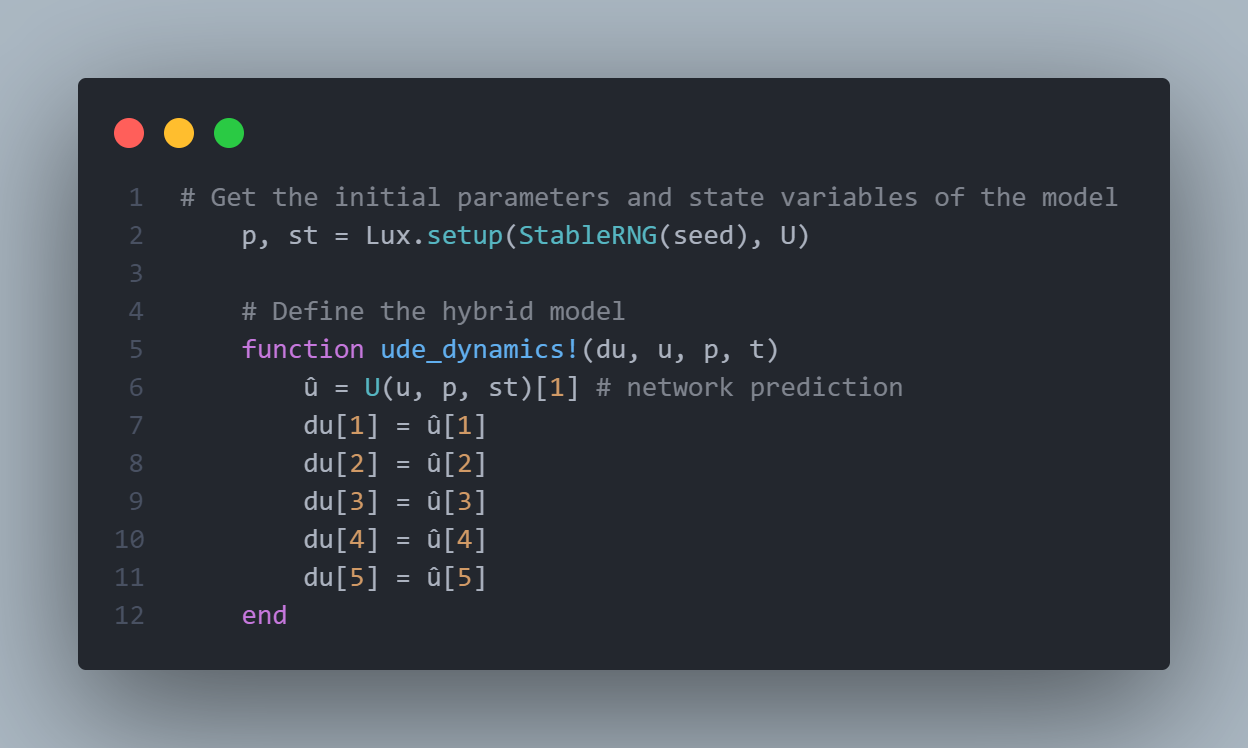
\includegraphics[width=\textwidth]{img/hibrid_model.png}
	\captionof{figure}{Modello ibrido che utilizza l'idea di rete neurale insieme all'idea di ODE}
	\label{fig:hibrid_model}
\end{minipage}

L'utilizzo successivo del modello di NN precedentemente introdotto \ref{fig:lux_nn} viene fatto 
utilizzandolo all'interno di un sistema di ODE. Questo viene utilizzato come predittore 
dei valori attualmente non conosciuti che modificano il sistema. Si puo' notare come non esista un 
vero e proprio aggiornamento dei pesi della rete, questo perche' i pesi sono implicitamente i parametri
del sistema di ODE e ogni iterazione li aggiorna per definizione.

\subsubsection*{Raffinazione con SINDy}

\subsubsection*{Utilizzo GPU}

\subsubsection{Applicazione Regole di Intervento}

\subsubsection*{Intervento Locale}
Descrizione delle regole e policy-like applicate al 
singolo nodo per cercare di ridurre la pandemia in quello 
specifico punto.

\subsubsection*{Intervento Globale}
Descrizione delle regole e policy-like applicate all'intero
modello (prevalentemente alla possibilità di migrare tra nodi)
per contenere il contagio a quanti meno nodi possibile.

Questo approccio è molto simile a quello che è stato un lockdown 
generalizzato applicato durante i primi mesi di pandemia durante la 
primavera 2020. 

\subsubsection{Applicabilità al mondo reale}
Descrizione di come applicare queste tecniche e policy richieda
un attento studio della causalità degli eventi, e un altrettanto 
attento studio sull'efficacia di un intervento piuttosto che di un altro.

E' chiaro quindi che attualmente le tecniche mostrate siano più 
a fine dimostrativo che a fine pratico.

Risultati grafici.

Bug e problematiche